\section{Results}

\subsection{Scenario analysis}

Figure \ref{fig:scenarios_overview} shows the range of results, measured by utility or the proportion of patients with an outcome of mRS 0-2, separating the changes for nLVO and LVO. Across all scenarios MSUs are usually found to be advantageous compared with usual care, but in some scenarios (comparing the best likely usual care with the worst likely MSU care), MSUs were found to be disadvantageous compared with usual care. Across the majority of scenarios the benefit of MSU care over usual care was typicall (interquartile range across scenarios) an improvement of 0.005 to 0.021 in utility for nLVO, and 0.016-0.052 for LVO treated with both IVT and MT. This translated to an improvement of the proportion of patients mRS 0-2 of 0.005-0.023 for nLVO, and 0.017-0.055 for LVO treated with both IVT and MT. The benefit to patients with LVO was derived mostly by improving benefit of MT by direct transport to a MT-capable unit.


\begin{figure}[h]
    \centering
    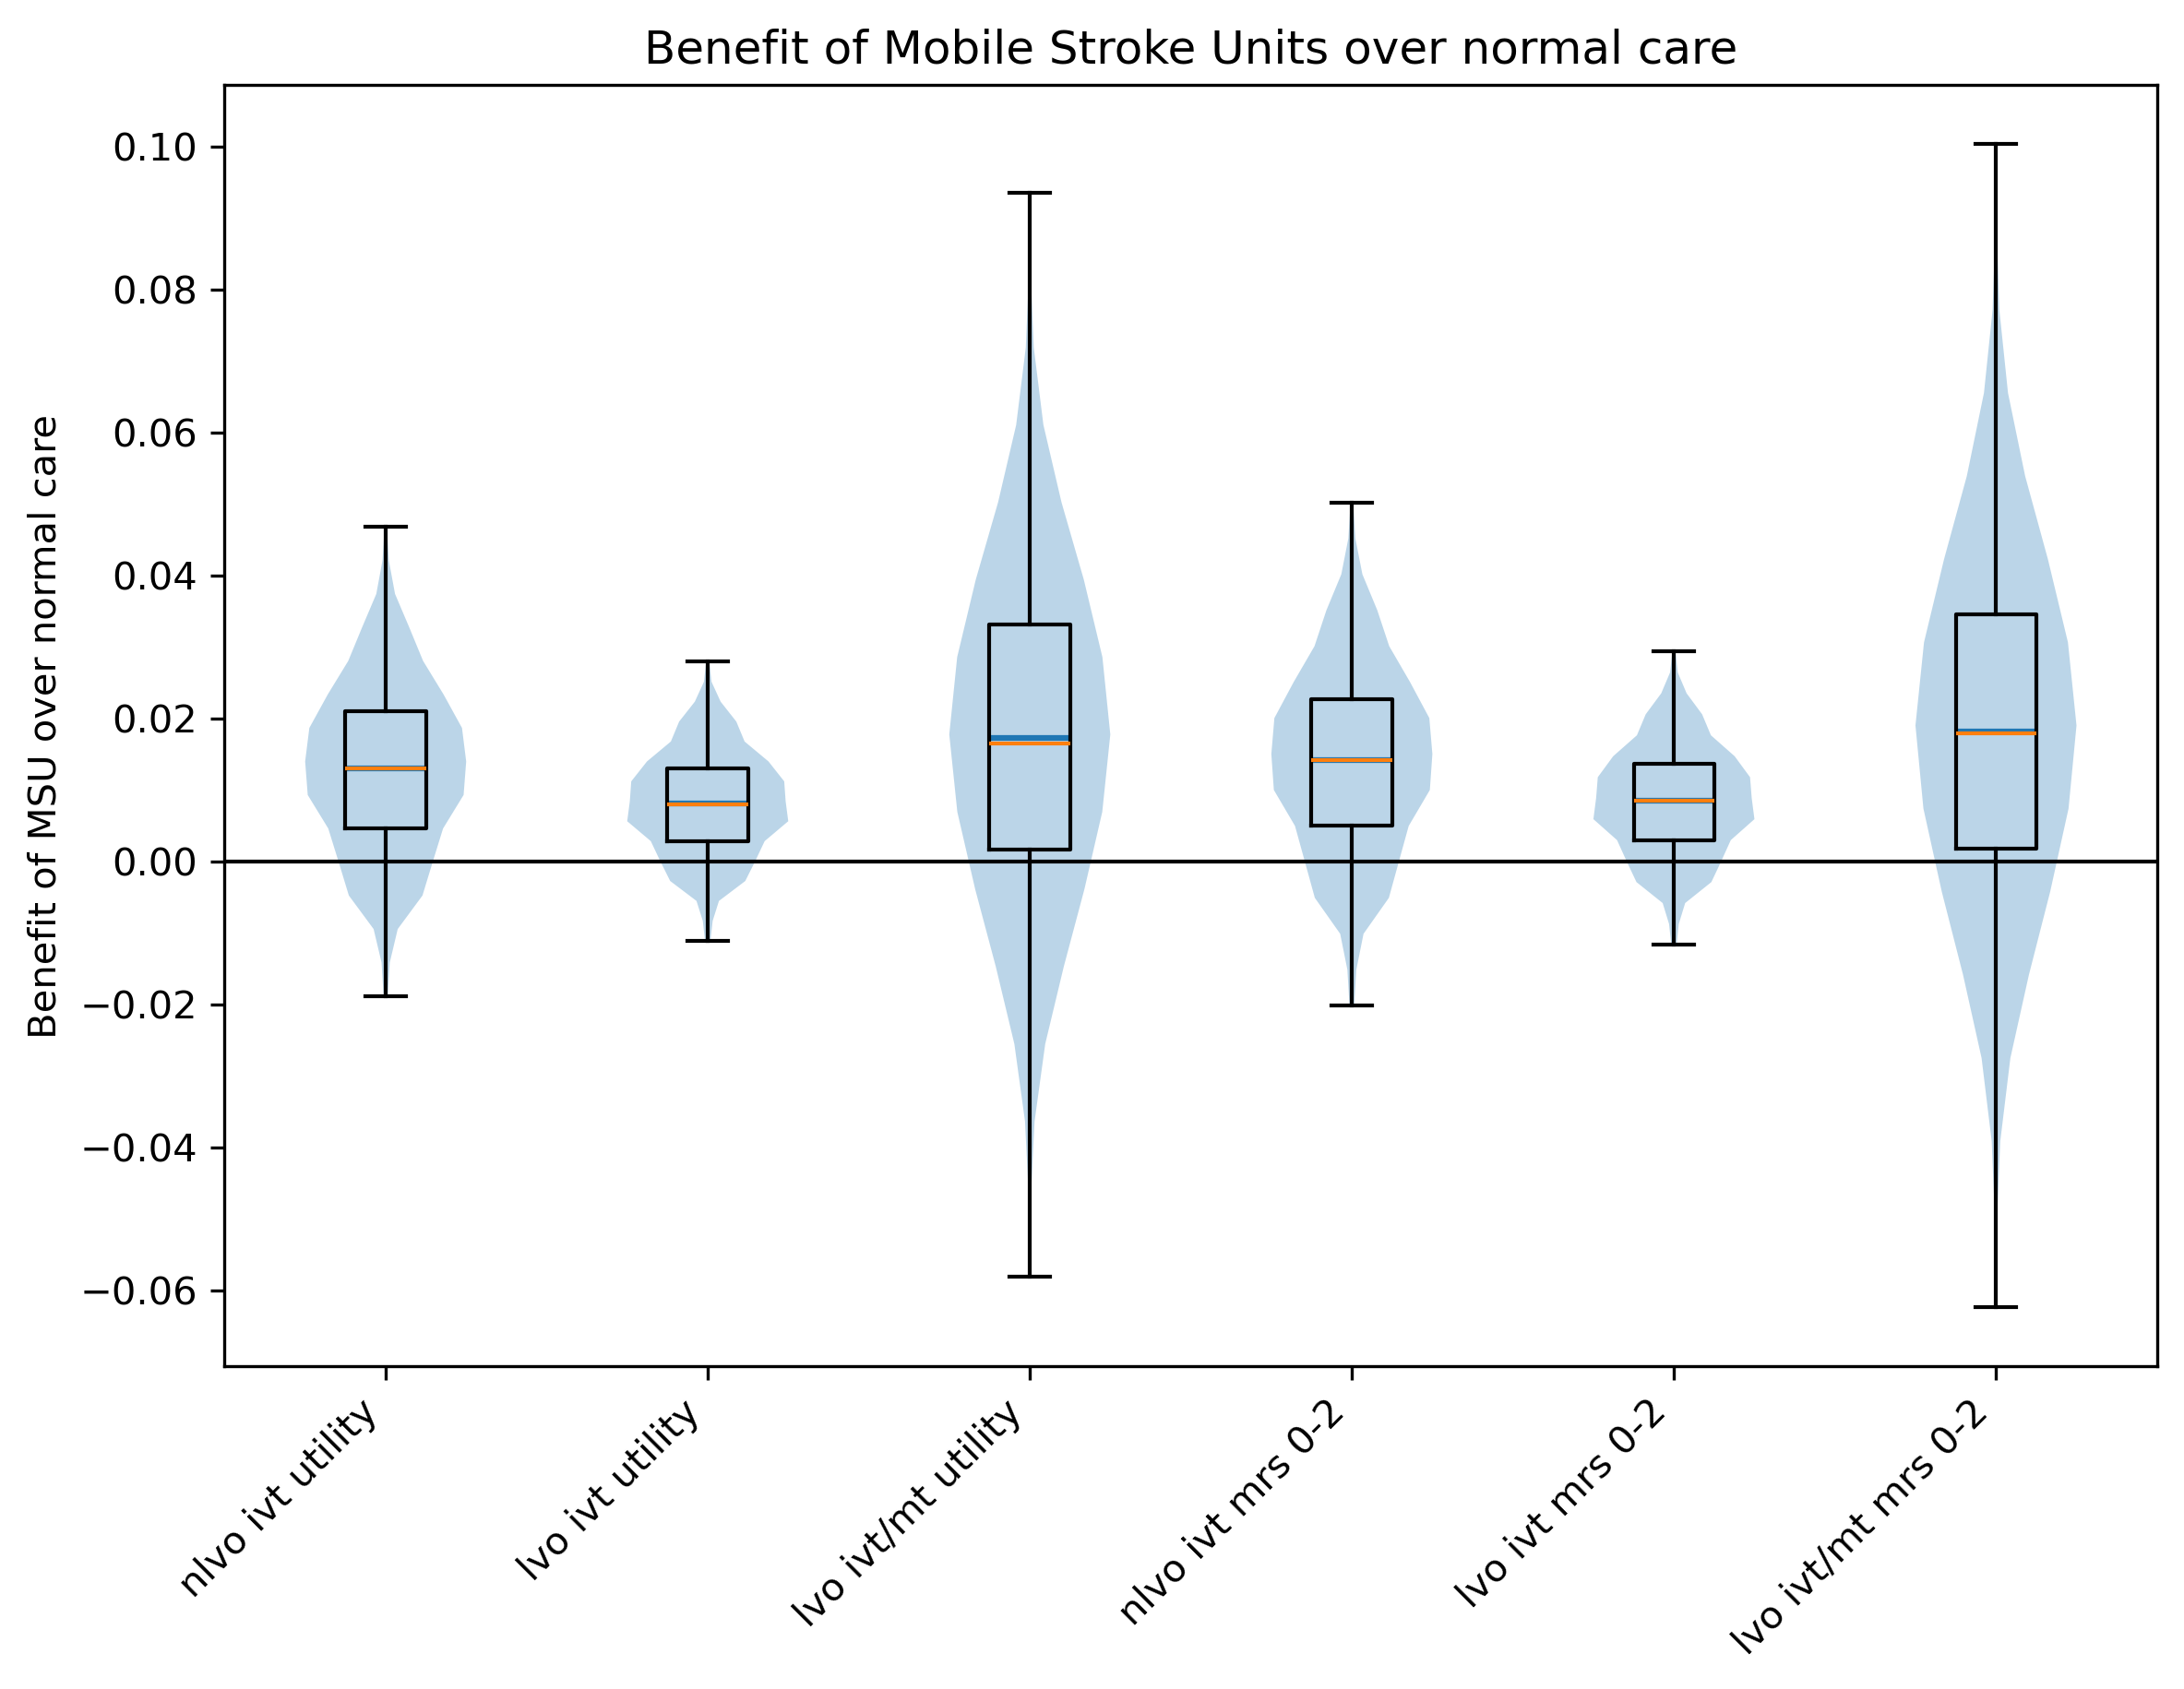
\includegraphics[width=0.6\linewidth]{images/scenario_results_summary.png}
    \caption{Benefit of usual care over MSU care across all scenarios, in the treated population, measured by utility or the proportion of patients with an outcome of mRS0-2, separating the changes for nLVO and LVO. Results for LVO show the effect of MSUs on the benefit derived from IVT alone, or by IVT/MT in combination. Box plots show range, interquartile range, and median. Overlaid over the box plots are violin plots showing the distribution of results across all scenarios. A positive value indicates MSUs provide an advantage over usual care, and a negative result show MSUs are disadvantageous compared with usual care. Results are the average effect across all LSOAs in England.}
    \label{fig:scenarios_overview}
\end{figure}

Figure \ref{fig:scenarios_utility} shows how changing model parameters affects the predicted benefit of MSUs, using utility as a measure. Results show the combined affect on nLVO/LVO assuming 70\% nLVO and 30\% LVO  in the treatable population. Changing time from onset to call only had marginal effect on the benefit of MSUs over usual care. Changing parameters that worsen usual care (such as lengthening ambulance response times, or lengthening arrival to IVT, lead to improved advantages of MSUs over usual care. Likewise, changing parameters that improve MSU care (such as MSU dispatch times, or time to IVT on scene) improved advantages of MSUs over usual care.

\begin{figure}[h]
    \centering
    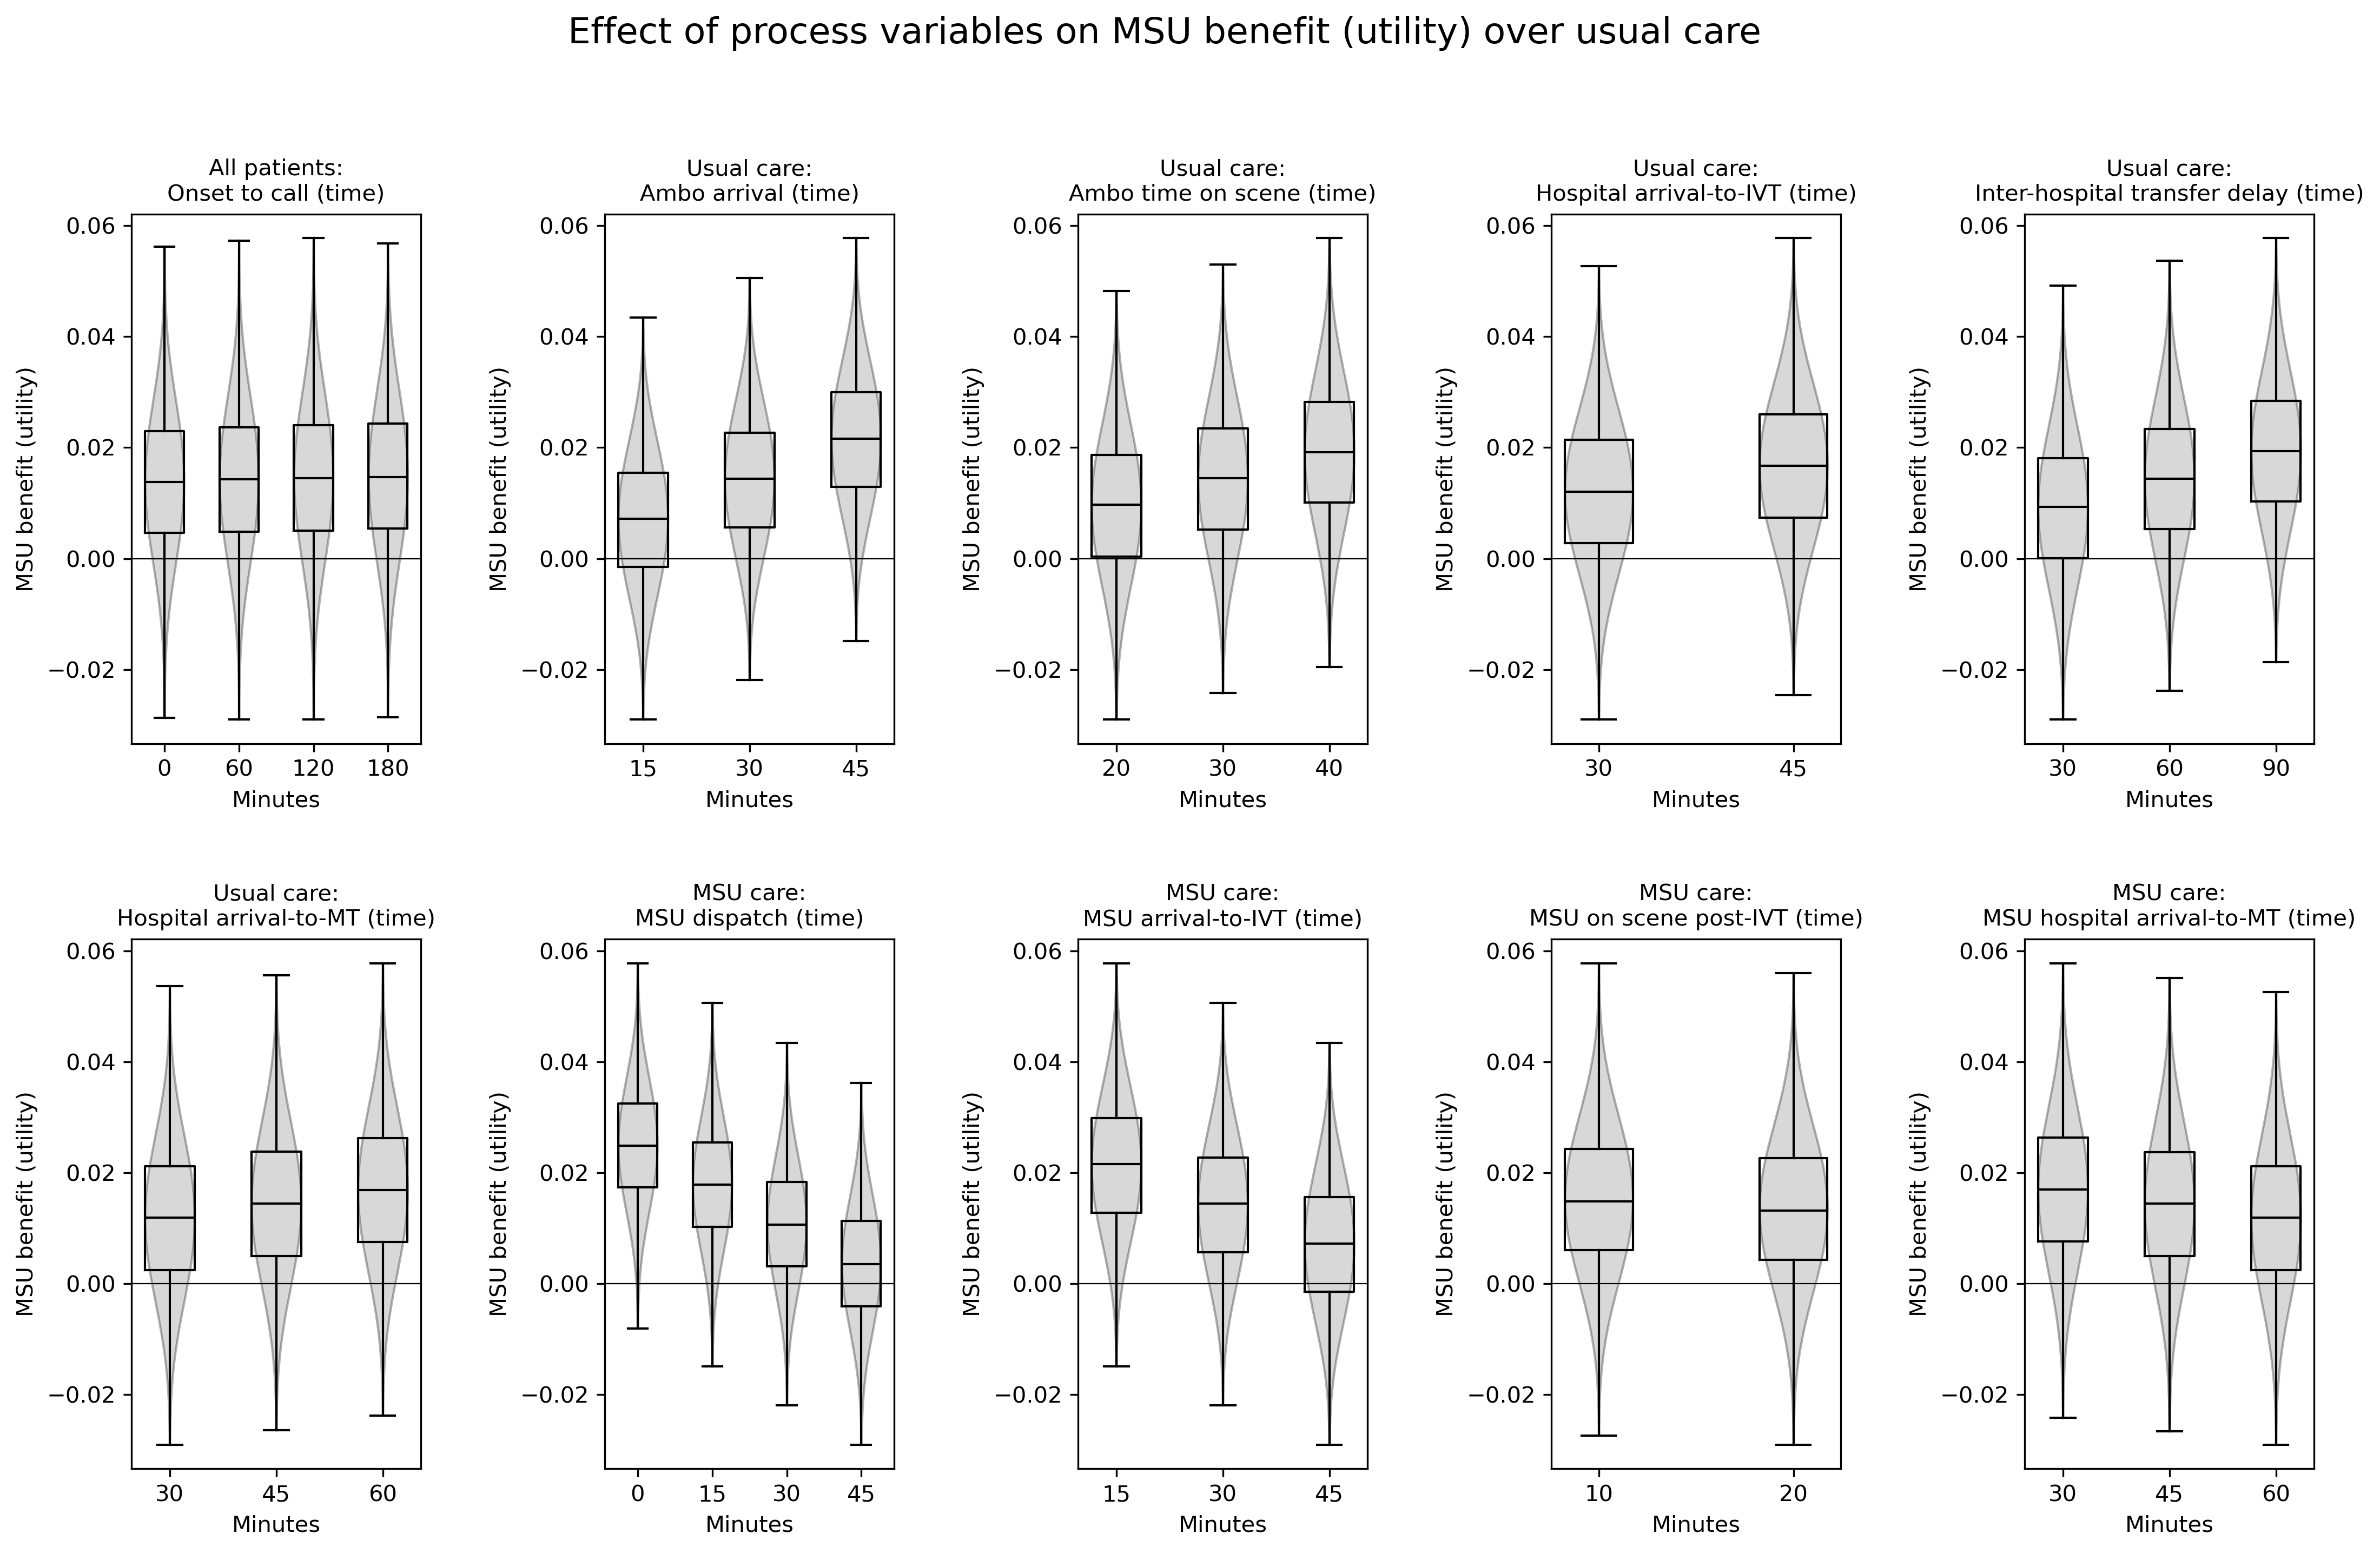
\includegraphics[width=1\linewidth]{images/msu_net_utility_benefit.png}
    \caption{The effect of changing model parameters on the predicted benefit of MSUs over usual care, in the treated population, measured by utility. For each target parameter results are averaged across all scenarios with that given parameter value. Box plots show range, interquartile range, and median. Overlaid over the box plots are violin plots showing the distribution of results across all scenarios. Results are the average effect across all LSOAs in England.}
    \label{fig:scenarios_utility}
\end{figure}

\subsection{Geographic variation}

In the base case scenario MSUs are based at comprehensive stroke centres only, and we assume there is a mix of 70\% nLVO and 30\% LVO in the treated population.

Figure \ref{fig:map_times} shows travel and transfer times for usual care and for MSUs. When a patient first attends an IVT-only centre, the times to IVT include the travel time to the IVT-only centre, the inter-hospital travel time, and a net additional delay of 60 minutes. There is significant variation in travel times to IVT centres, but there is more substantial variation in times to MT due to the need for transfer. 67\% of LSOAs and 70\% of admissions require transfer for MT. As, the base MSUs are based at comprehensive stroke centres only, travel times for a MSU can exceed the travel time of a normal ambulance to the closest centre providing IVT, and this extra travel time can lead to delayed time to IVT in those regions furthest away from MSU bases locations.

\begin{figure}[h]
    \centering
    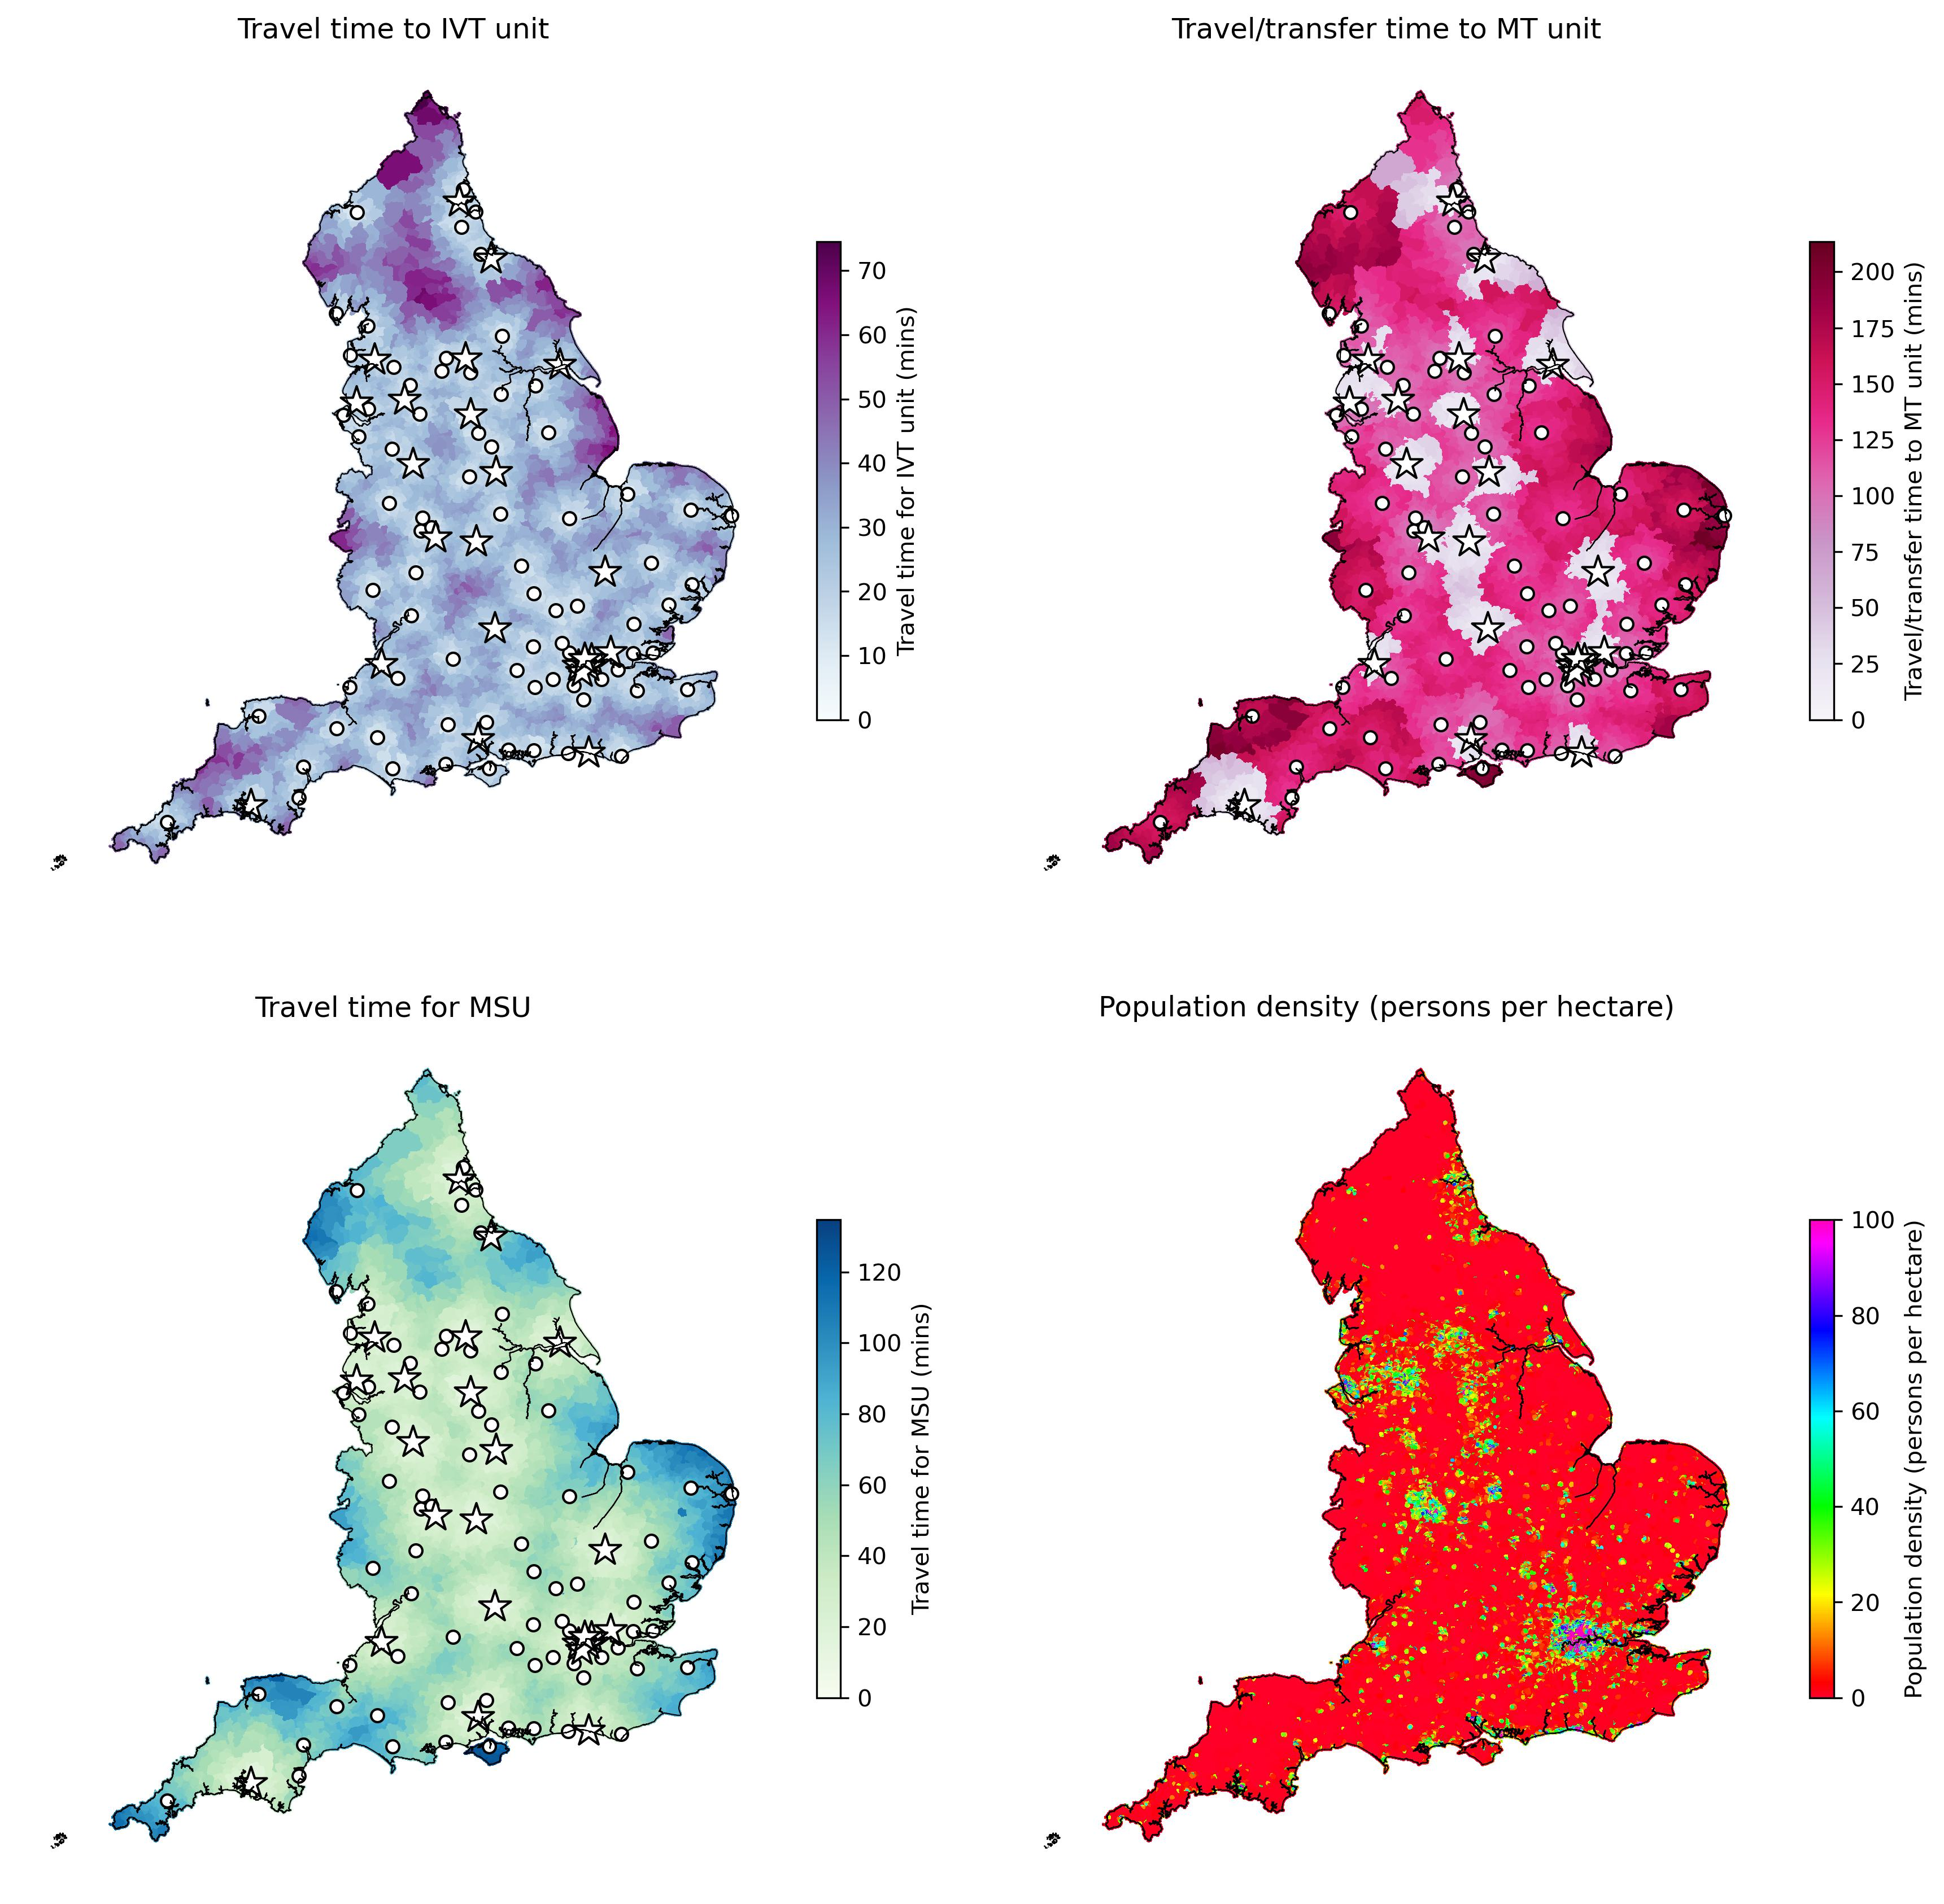
\includegraphics[width=1.0\linewidth]{images/map_times.jpg}
    \caption{Travel times for each LSOA. \textit{Left}: Travel times to nearest unit providing IVT. \textit{Middle}: Travel times to unit providing MT. For those first attending an IVT-only centre, the travel times include the travel time to the IVT-only centre, the inter-hospital travel time, and a net additional delay of 60 minutes. \textit{Right}: Travel times for MSUs. Circles show locations of IVT-only units. Stars show locations of comprehensive stroke centres providing both IVT and MT, and being the base locations of MSUs.}
    \label{fig:map_times}
\end{figure}


In this base case, without reperfusion treatment, there is an average outcome utility of 0.52 across nLVO and LVO. With usual care, the is a utility gain of 0.086 in treated patients. MSUs provided an average further utility gain in treated patients of 0.022 over usual care.

Figure \ref{fig:msu_map_utility} shows maps of geographic variation in benefit of MSUs over usual care, by stroke type, using the reasonable base case scenario. Figure \ref{fig:msu_histograms} shows the distribution of net benefit (assuming 70\%nLVO, 30\% LVO in the treated population) across LSOAs. There is significant variation in the benefit of reperfusion using usual care, with those living closest to comprehensive stroke units receiving the greatest benefit. This is due the larger utility gain of reperfusion treatment coming from the treatment of LVO, and with those patients benefiting most from rapid access to thrombectomy.

The benefit of MSUs over usual care follows different patterns for nLVO and LVO. For nLVO, the benefit of MSU falls with distance away from the MSU base. For LVO the benefit first falls with with distance away from the MSU base, but then benefit increases where use of the MSU avoids inter-hospital transfer for MT, before falling again with greater travel times for the MSU. The catchment area of benefit for LVO, when using MSUs, is therefore wider than the catchment area of benefit for nLVO, with the maximum benefit being in a halo a little way away from the MSU base location, where patient transfer for MT is avoided but MSU travel times are still acceptable.


\begin{figure}[h]
    \centering
    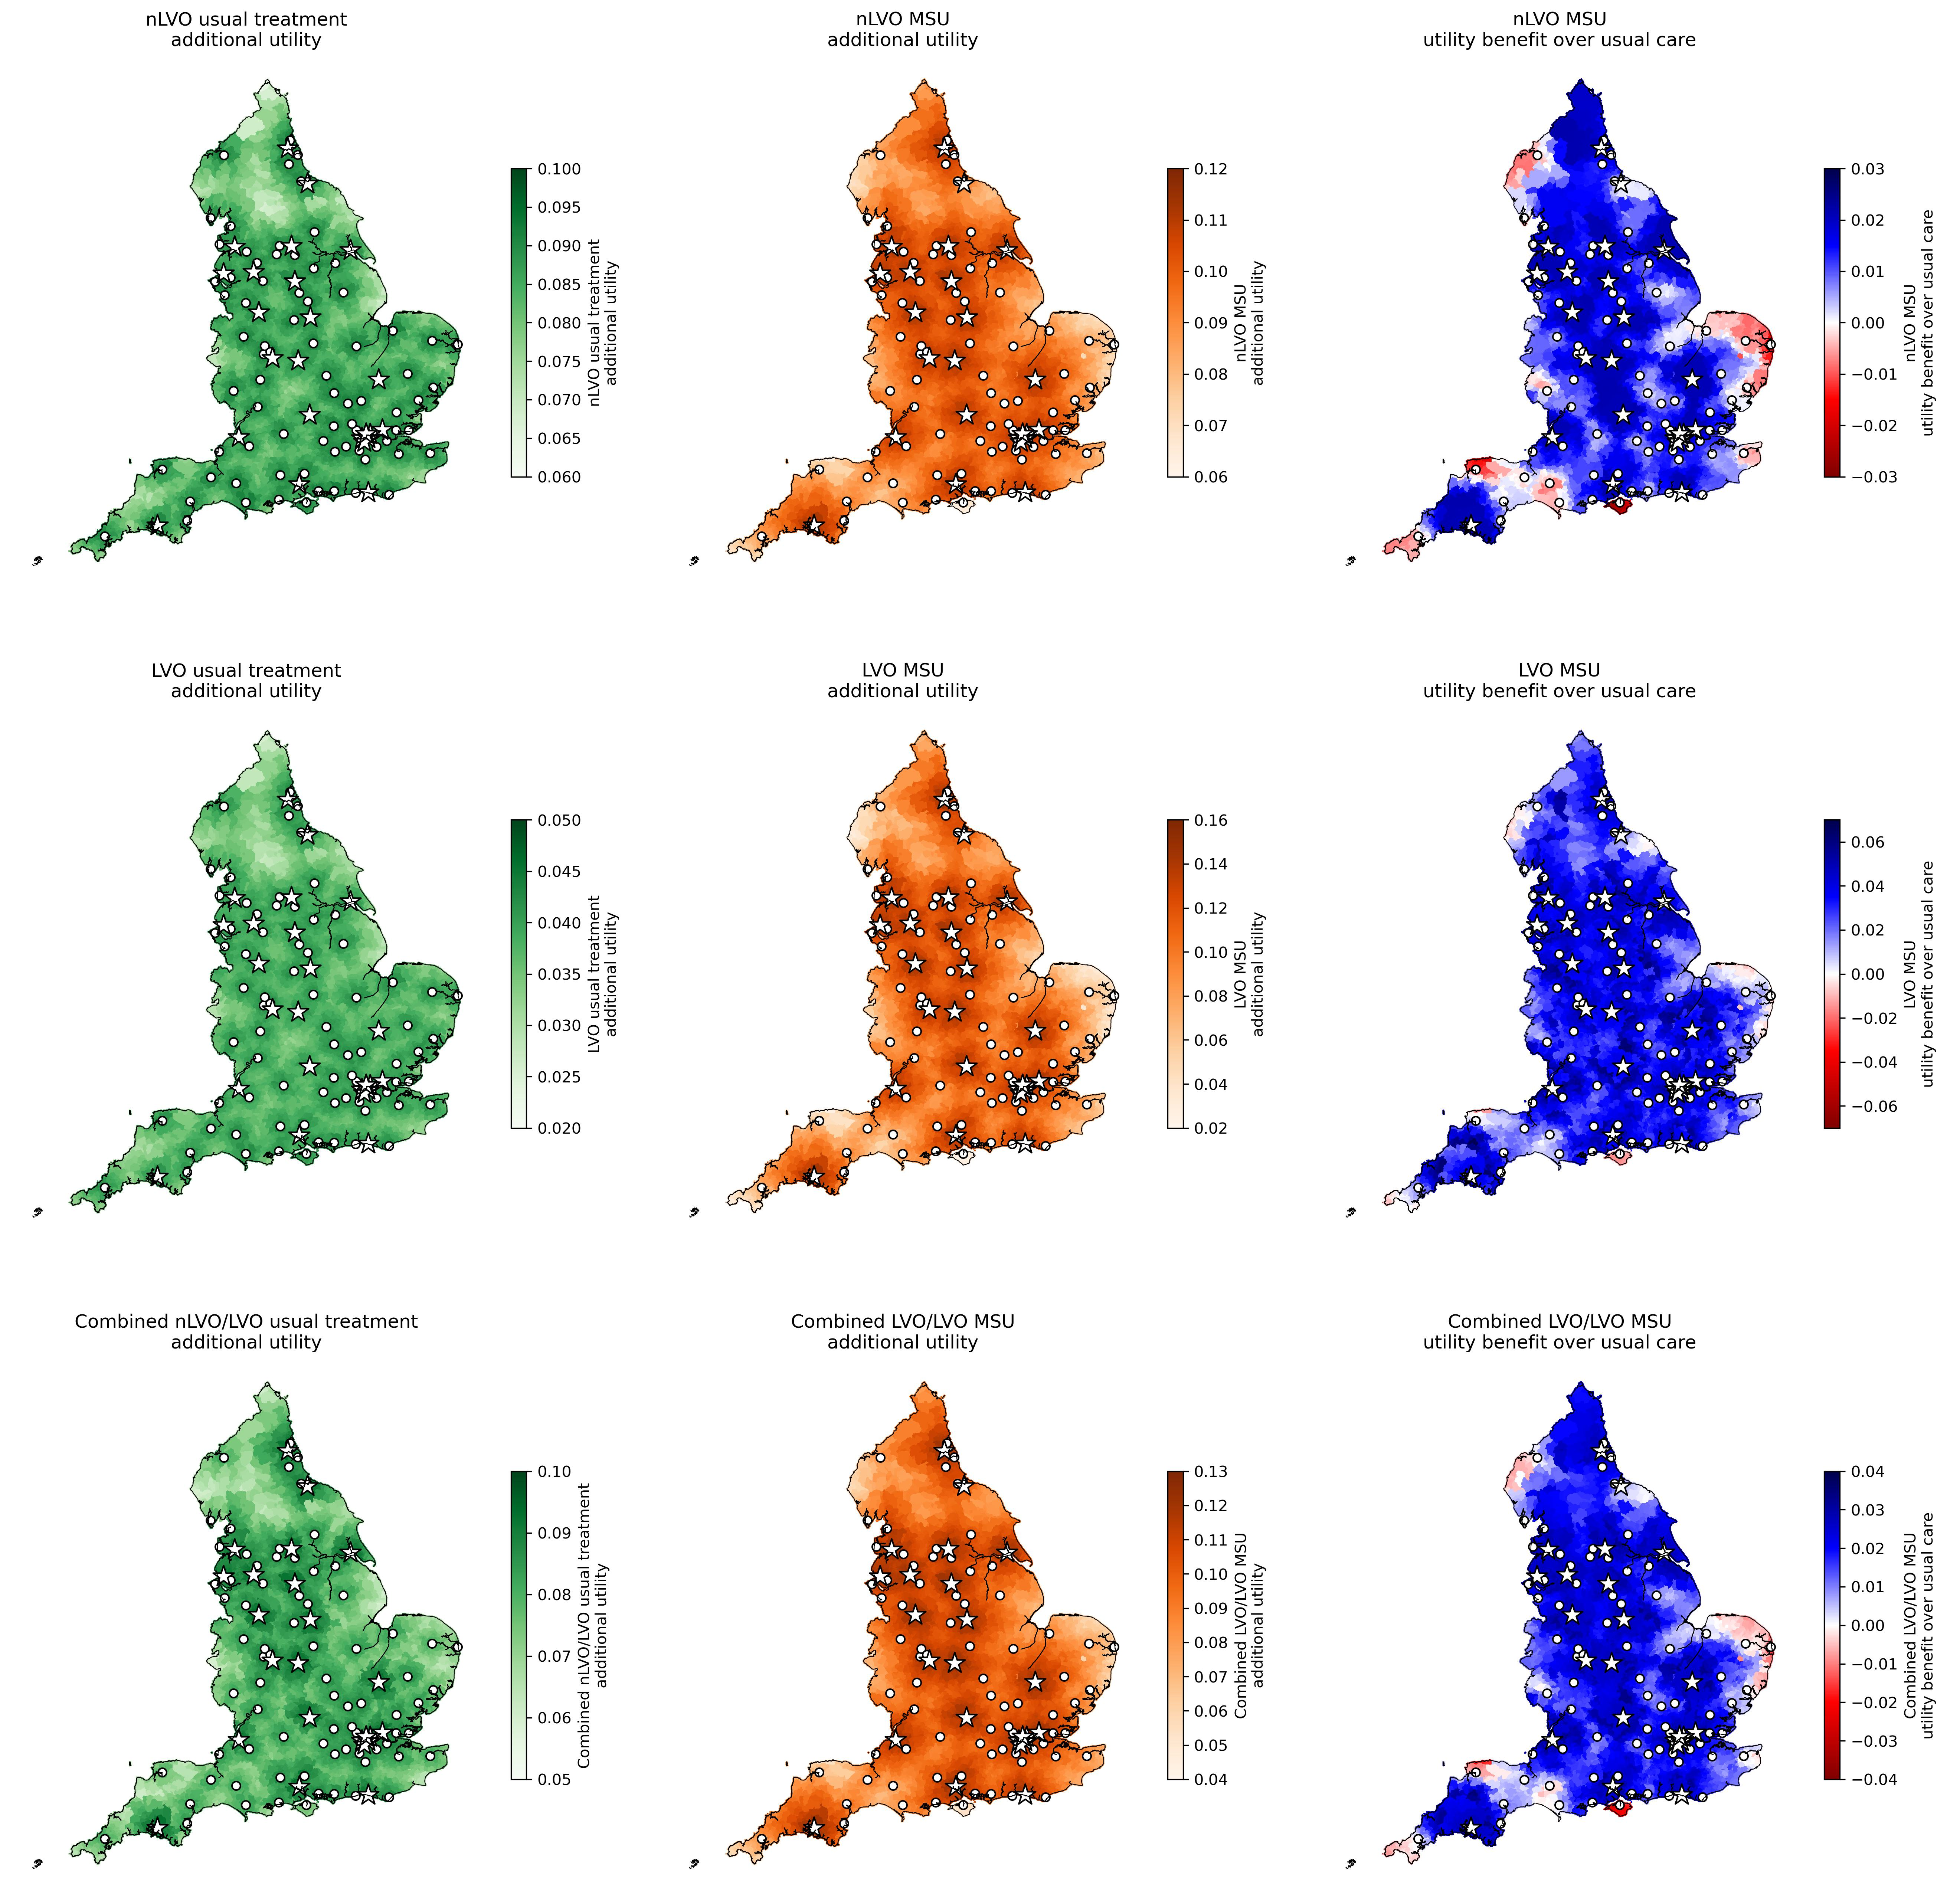
\includegraphics[width=1\linewidth]{images/map_utility.jpg}
    \caption{Map of treatment benefits, calculated by LSOA for the treated population. \textit{Top}: Treatment of nLVO; \textit{Middle}: Treatment of LVO, \textit{Bottom}: Combination of treatment (based on 70\% nLVO and 30\% LVO in the treated population). \textit{Left (green)}: Benefit of usual care over no treatment;\textit{Middle (orange)}: Benefit of MSU care over no treatment; \textit{Right (blue/red)}: Benefit of MSU care over usual care. Circles show locations of IVT-only units. Stars show locations of comprehensive stroke centres providing both IVT and MT, and being the base locations of MSUs.}
    \label{fig:msu_map_utility}
\end{figure}

Figure \ref{fig:msu_histograms} shows histograms of benefit of MSUs over usual care. For most LSOAs MSU improve time to IVT and MT, but some areas have worsened times. This is reflected in most areas having a benefit of about a 0.03 increase in the proportion of patients with MRS 0-2 after stroke, and similarly a benefit of about a 0.03 increase in utility after stroke. Some areas though have reduced benefit, or even disbenefit of using MSUs. The maximum benefit is about 0.04 improvement in both the proportion of patients with MRS 0-2 after stroke and utility after stroke.

\begin{figure}[h]
    \centering
    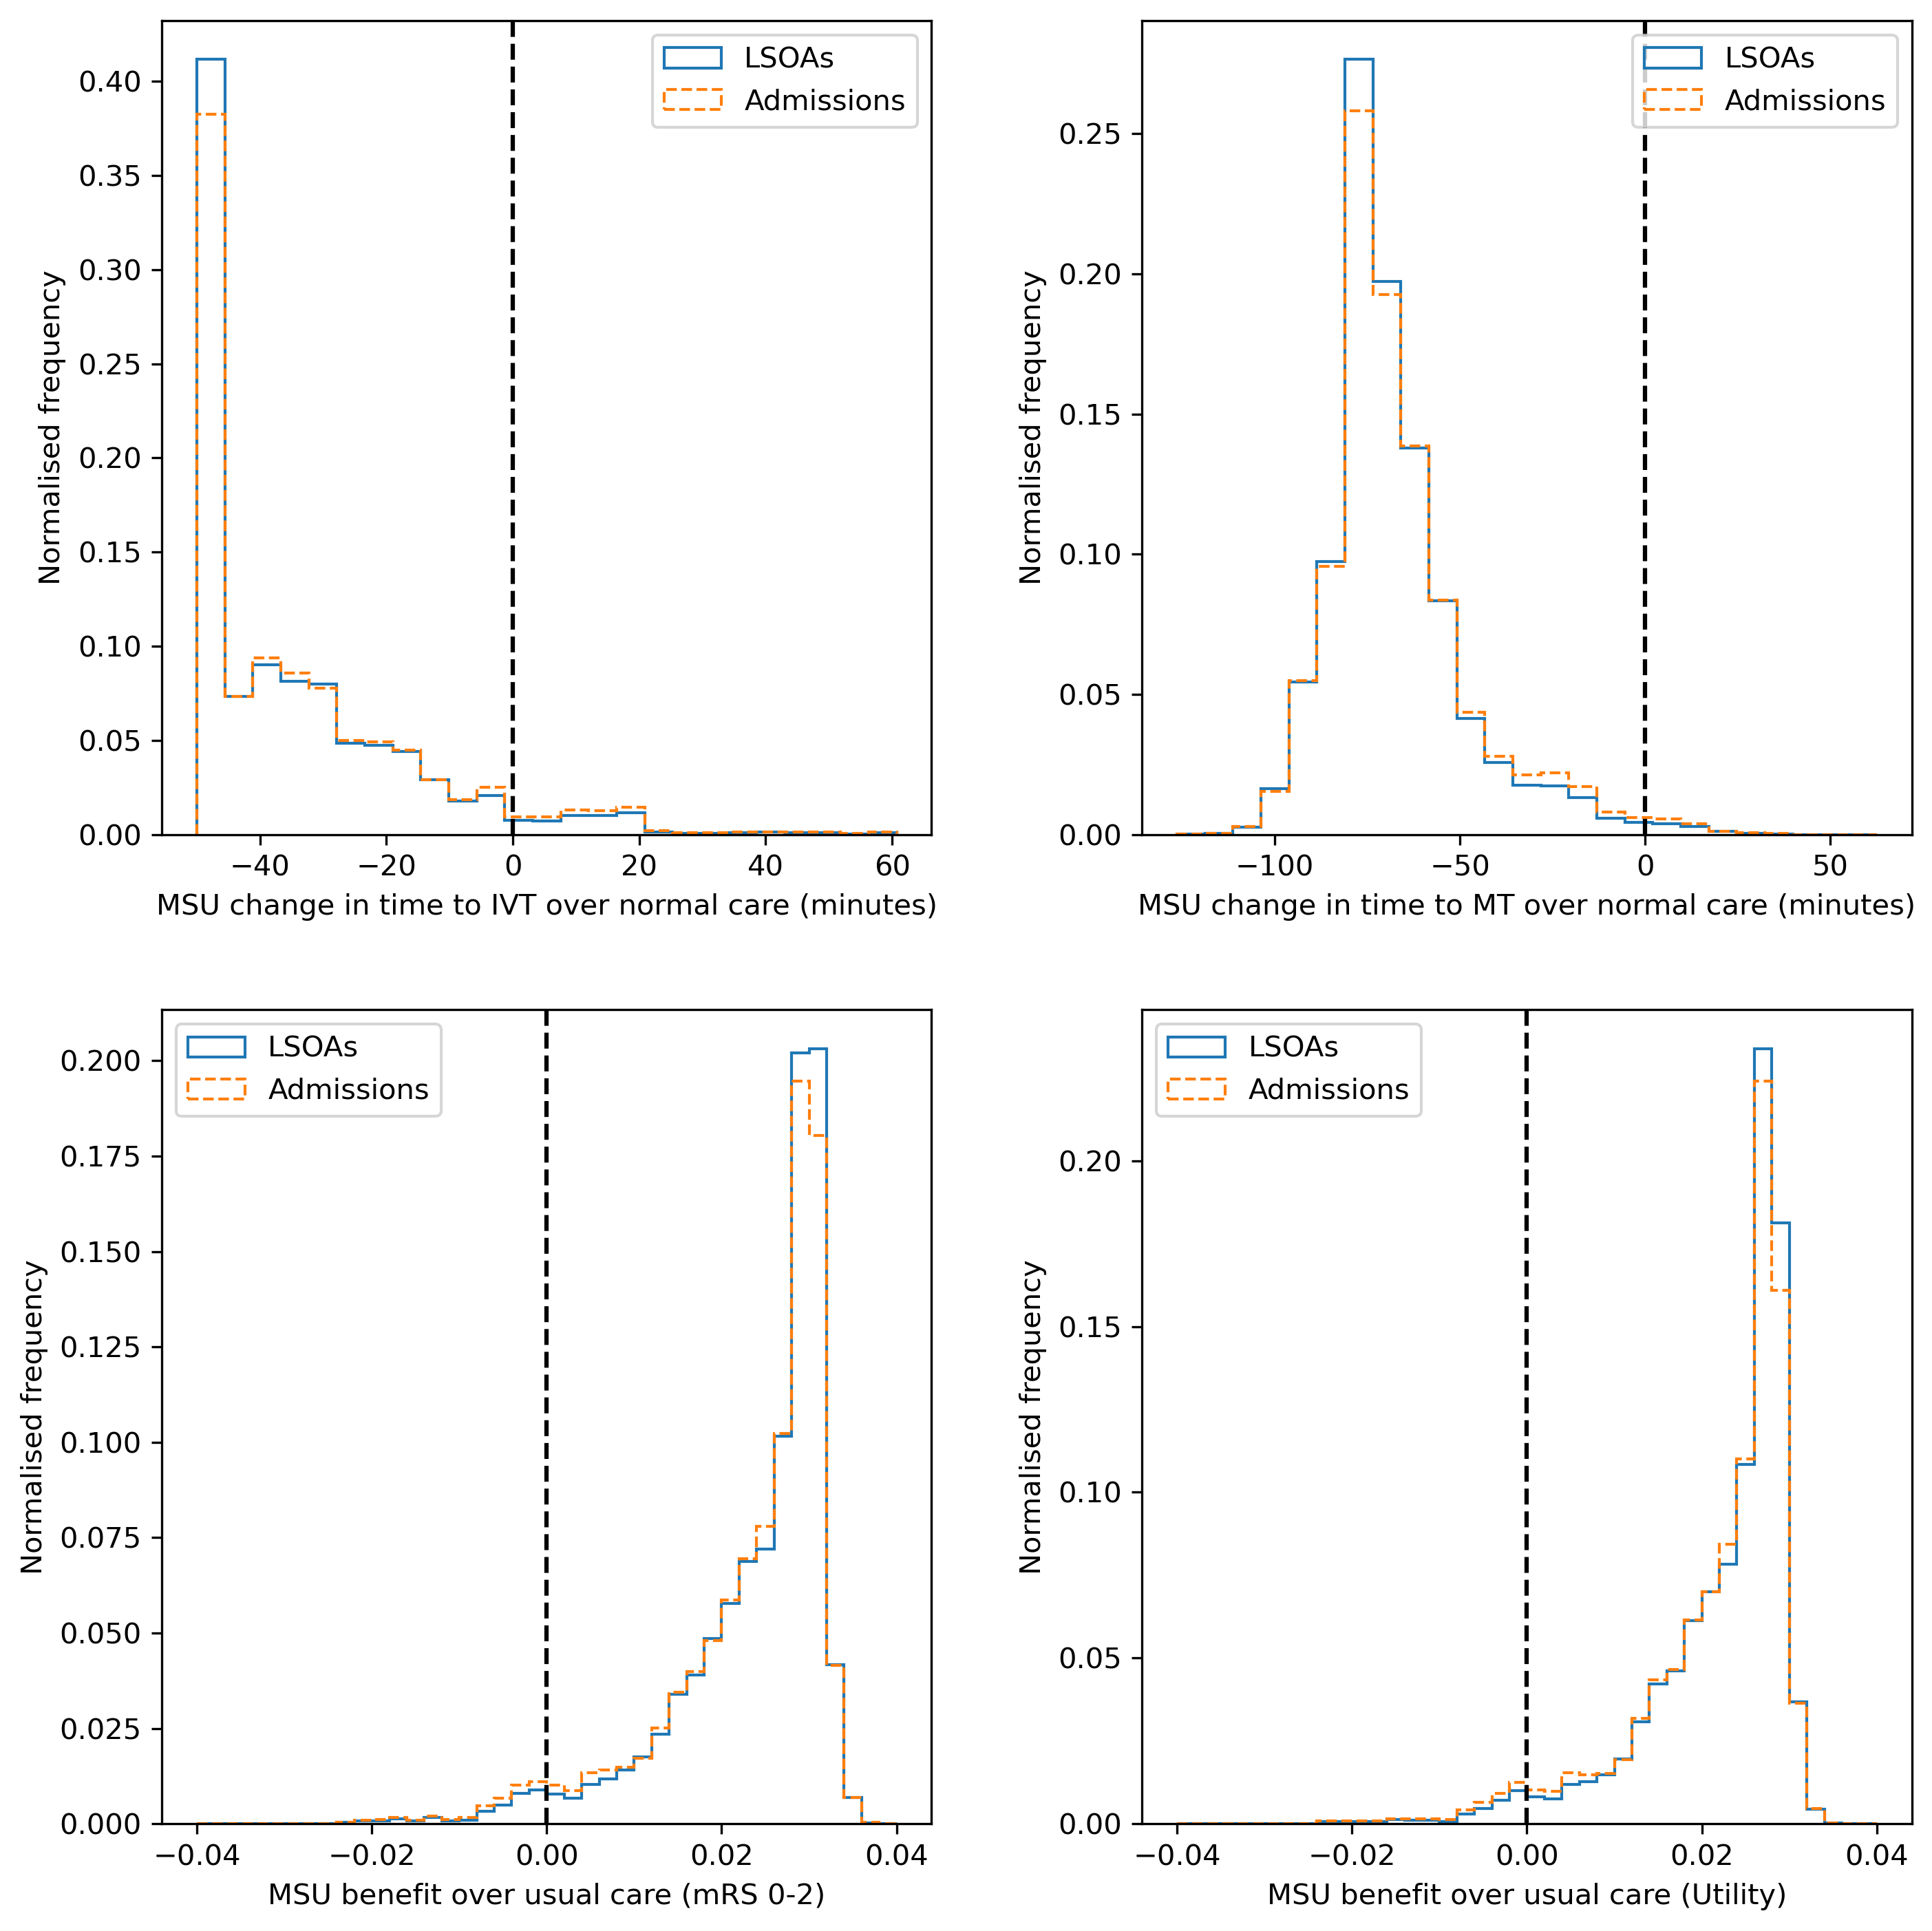
\includegraphics[width=0.75\linewidth]{images/histograms.png}
    \caption{Distribution of benefit of MSUs over normal care across MSUs. Benefit is described either as even across LSOAs (solid line), or weighted by admissions by LSOA (dotted line). Histograms show change in time to IVT (top left), time to MT (top right), proportion mRS 0-2 (bottom left), or utility (bottom right).}
    \label{fig:msu_histograms}
\end{figure}

\subsection{Varying number of MSU locations}

A greedy algorithm was used to select locations of MSUs. The utility gain is calculated for those patients treated by a MSU rather than usual care. As the number of MSU locations increased, the benefit of MSUs over usual care increased (\ref{fig:greedy}), but with diminishing returns. The advantage of MSU care over usual care improved utility by 0.020, 0.024, 0.027, and  with 10, 25, 50 and 100 MSU base locations. 

When selecting locations of mobile stroke units, in the first 10 selections, 3 were comprehensive stroke units, and in the first 20, 8 were comprehensive stroke units.

\begin{figure}[h]
    \centering
    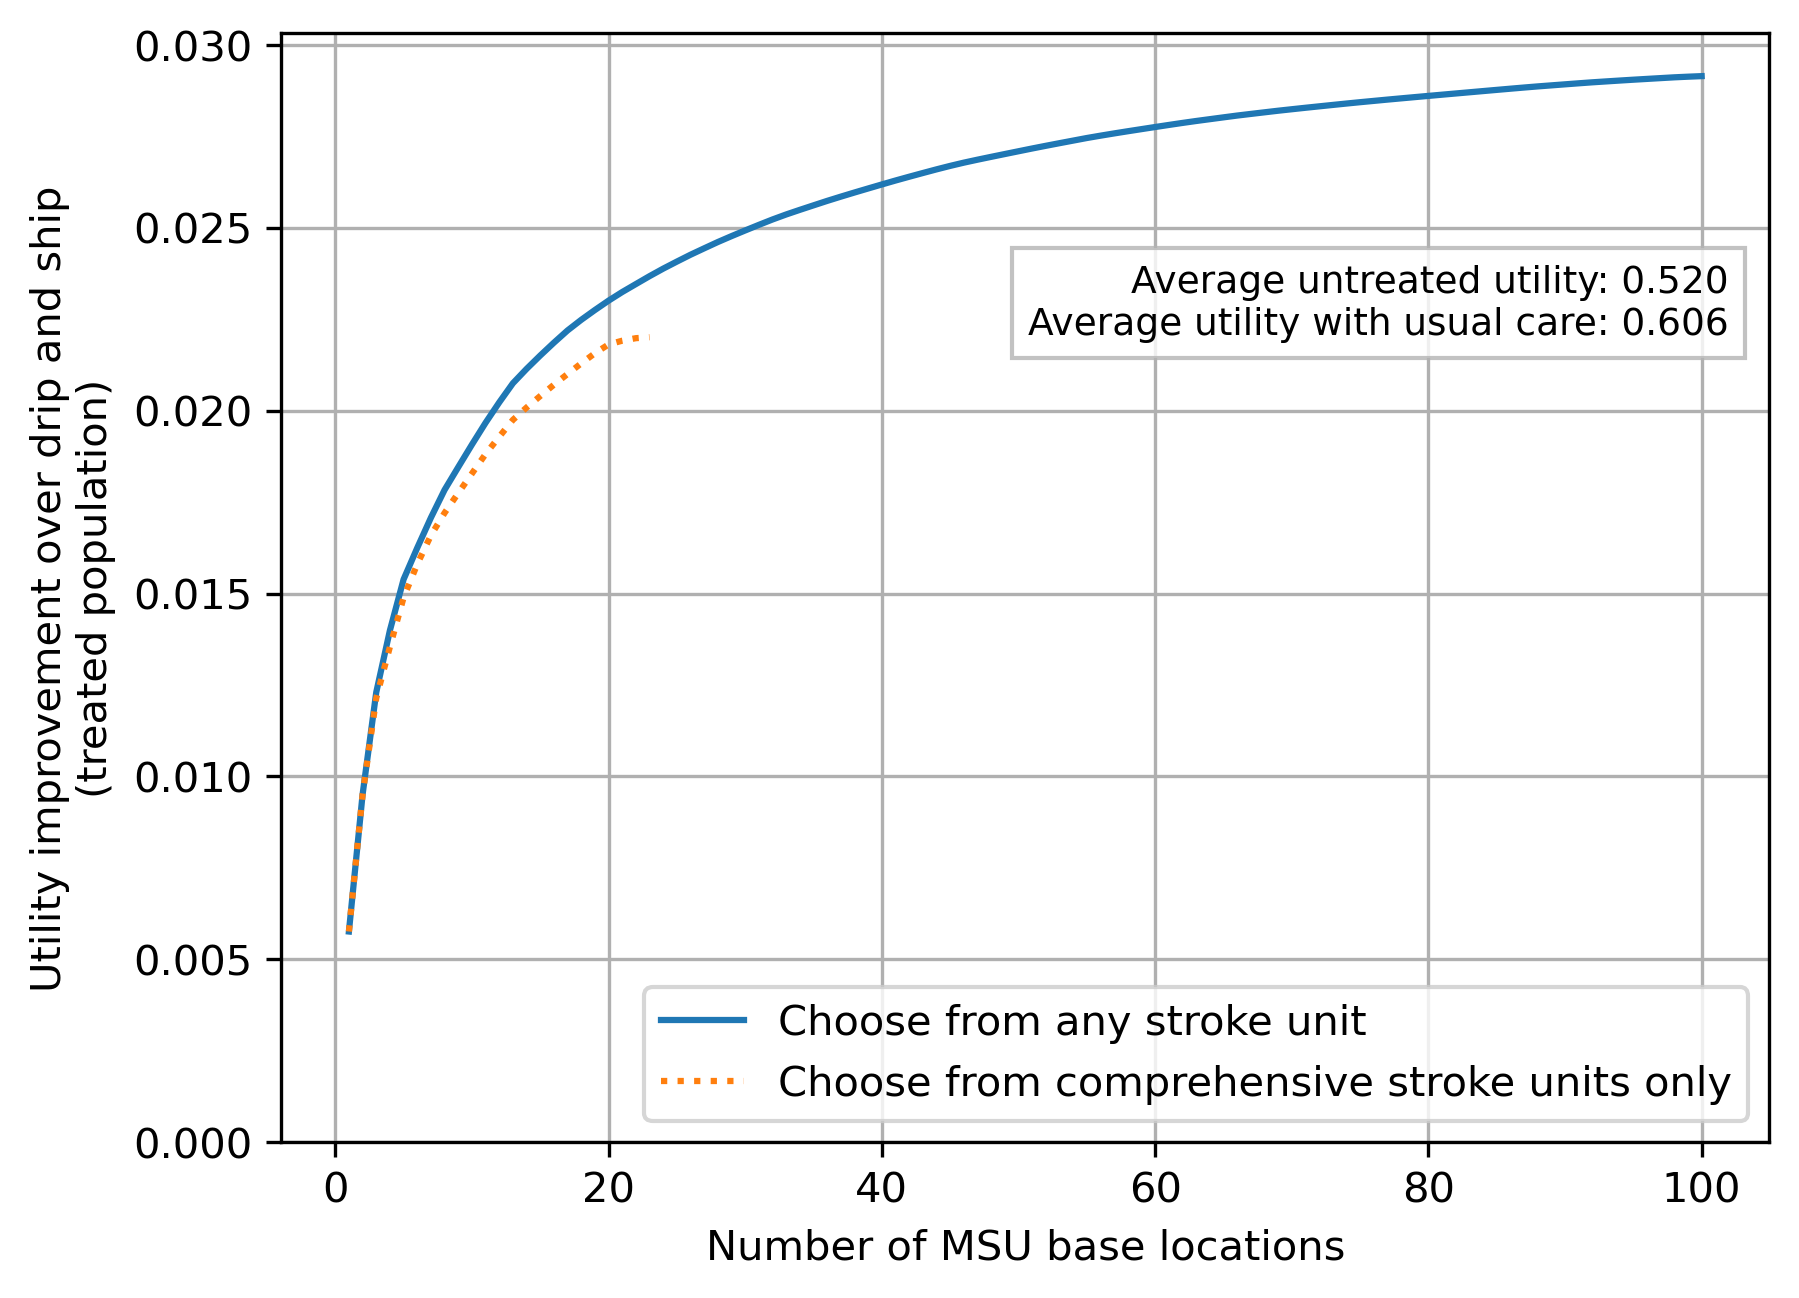
\includegraphics[width=0.5\linewidth]{images/msu_advantages_greedy.png}
    \caption{Increasing number of base locations of MSUs, with selection by a greedy algorithm based on improvements in utility. The utility improvement is for those patients treated by MSU rather than usual care.}
    \label{fig:greedy}
\end{figure}


